% Author: Dominik Harmim <harmim6@gmail.com>


\documentclass[10pt, xcolor=pdflatex, hyperref={unicode}, aspectratio=169]{beamer}


\usepackage{newcent}
\usepackage[utf8]{inputenc}
\usepackage[british]{babel}
\usepackage[T1]{fontenc}
\usepackage{xcolor}
\usepackage{listings}
\usepackage{appendixnumberbeamer}
\usepackage{multirow}
\usepackage{mathtools}

% Setting of a path to the pictures.
\graphicspath{{img/}}

\definecolor{bluekeywords}{rgb}{.13, .13, 1}
\definecolor{greencomments}{rgb}{0, .5, 0}
\definecolor{redstrings}{rgb}{.9, 0, 0}

\lstset{
    basicstyle=\ttfamily,
    keywordstyle=\color{bluekeywords},
    commentstyle=\color{greencomments},
    stringstyle=\color{redstrings},
    backgroundcolor=\color{yellow!10},
    language=c++,
    tabsize=2,
    escapeinside={<@}{@>},
    frame=trBL,
    columns=fullflexible,
    showstringspaces=false,
    keepspaces=true,
    showspaces=false,
    showtabs=false,
    breaklines=true,
    breakatwhitespace=true
}


%%%%%%%%%%%%%%%%%%%%%%%%%%%%%%%%%%%%%%%%%%%%%%%%%%%%%%%%%%%%%%%%%%%%%%%%%%%%%%%%


\usetheme{FIT}

\title[Advanced Static Analysis of Atomicity in Concurrent Programs through Facebook Infer]{Advanced Static Analysis of Atomicity in Concurrent Programs through Facebook Infer}
\subtitle{Master's Thesis}

\author{\texorpdfstring{%
    Dominik Harmim \\
    \footnotesize{Supervisor: prof. Ing. Tomáš Vojnar, Ph.D.}%
}{Dominik Harmim; Supervisor: prof. Ing. Tomáš Vojnar, Ph.D.}}

\institute{%
    xharmi00@stud.fit.vutbr.cz \\
    Brno University of Technology, Faculty of Information Technology%
}

\subject{Master's Thesis Defence}

\date{\today}


%%%%%%%%%%%%%%%%%%%%%%%%%%%%%%%%%%%%%%%%%%%%%%%%%%%%%%%%%%%%%%%%%%%%%%%%%%%%%%%%


\begin{document}


%%%%%%%%%%%%%%%%%%%%%%%%%%%%%%%%%%%%%%%%%%%%%%%%%%%%%%%%%%%%%%%%%%%%%%%%%%%%%%%%


\section{Title Slide}
\frame[plain]{\titlepage}


%%%%%%%%%%%%%%%%%%%%%%%%%%%%%%%%%%%%%%%%%%%%%%%%%%%%%%%%%%%%%%%%%%%%%%%%%%%%%%%%


\section{Motivation}
\begin{frame}[fragile]{Motivation}
    \textbf{The goal:} \emph{improve detection} of \alert{atomicity violations} within \emph{Facebook Infer}.
    
    \bigskip

    \begin{itemize}
        \item Detecting and checking desired \alert{atomicity} of \emph{function call sequences}.
            \medskip
            \begin{itemize}\setlength\itemsep{.8em}
                \item Often required in \emph{concurrent programs}.

                \item \alert{Violation} may cause \emph{nasty errors}.
            \end{itemize}
    \end{itemize}

    \vfill

    \begin{columns}
        \begin{column}{.6 \linewidth}
            \centering
\begin{lstlisting}
void invoke(char *method) {
  <@\texttt{\ldots}@>
  if (server.<@\textbf{is\_registered}@>(method)) {
    server.<@\textbf{invoke}@>(method);
  }
  <@\texttt{\ldots}@>
}
\end{lstlisting}
        \end{column}

        \begin{column}{.4 \linewidth}
            \centering

            The sequence of \texttt{\textbf{is\_registered}} and \texttt{\textbf{invoke}} should be \alert{executed atomically}.

            \bigskip

            \footnotesize{If \emph{not locked}, \texttt{\textbf{method}} can be unregistered by a~\emph{concurrent thread}.}
        \end{column}
    \end{columns}
\end{frame}


%%%%%%%%%%%%%%%%%%%%%%%%%%%%%%%%%%%%%%%%%%%%%%%%%%%%%%%%%%%%%%%%%%%%%%%%%%%%%%%%


\section{Facebook Infer}
\begin{frame}{Facebook Infer}
    \begin{columns}
        \begin{column}{1 \linewidth}
            \begin{itemize}
                \item Open-source \alert{static analysis framework} for \emph{interprocedural analyses}.
                    \medskip
                    \begin{itemize}
                        \item Based on \alert{abstract interpretation}.
                    \end{itemize}
            \end{itemize}
        \end{column}
        \hfill
    \end{columns}

    \medskip

    \begin{columns}
        \begin{column}{.55 \linewidth}
            \begin{itemize}\setlength\itemsep{2em}
                \item Highly \alert{scalable}.
                    \medskip
                    \begin{itemize}\setlength\itemsep{.8em}
                        \item Follows principles of \emph{compositionality}.

                        \item Computes function \emph{summaries} \alert{bottom-up} on call-trees.
                    \end{itemize}

                \item Supports C, C++, Java, Obj-C, C\#.
            \end{itemize}
        \end{column}

        \begin{column}{.45 \linewidth}
            \centering
            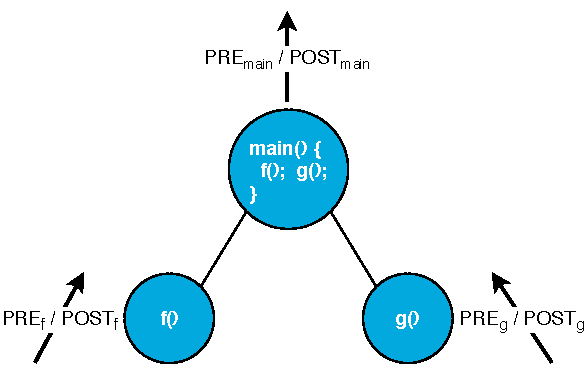
\includegraphics[width=1 \linewidth]{infer.pdf}
        \end{column}
    \end{columns}
\end{frame}


%%%%%%%%%%%%%%%%%%%%%%%%%%%%%%%%%%%%%%%%%%%%%%%%%%%%%%%%%%%%%%%%%%%%%%%%%%%%%%%%


\section{Atomer: Atomicity Violations Analyser}
\begin{frame}{Atomer: Atomicity Violations Analyser}
    \begin{itemize}\setlength\itemsep{1.5em}
        \item \alert{Facebook Infer plugin} created within the author's BSc thesis:
            \medskip
            \begin{thebibliography}{1}
                \bibitem[harmimBP]{harmimBP}
                \textsc{Harmim, D.} \textit{Static Analysis Using Facebook Infer to Find Atomicity Violations}. Brno, 2019. Bachelor's thesis. Brno University of Technology, Faculty of Information Technology. Supervisor \textsc{Vojnar, T.}
            \end{thebibliography}

        \item \textbf{Assumption}: \alert{call sequences} executed \emph{atomically once} should (probably) be executed \emph{always atomically}.

        \item Implemented for \emph{C~programs} that use \emph{PThread locks}.

        \item Limited \alert{scalability} on \emph{large codebases}.

        \item Reports many \alert{false alarms} when analysing \emph{real-life} code.
    \end{itemize}
\end{frame}


%%%%%%%%%%%%%%%%%%%%%%%%%%%%%%%%%%%%%%%%%%%%%%%%%%%%%%%%%%%%%%%%%%%%%%%%%%%%%%%%


\section{Proposed Atomer's Enhancements}
\begin{frame}{Proposed Atomer's Enhancements}
    \begin{itemize}\setlength\itemsep{2em}
        \item \emph{Approximating} \alert{sequences} of calls by \alert{sets} of calls (described later on). 

        \item Support for \alert{C++} and \alert{Java}.
            \medskip
            \begin{itemize}
                \item Working with \emph{advanced locks}: re-entrant locks, monitors, lock guards, etc.
            \end{itemize}

        \item Distinguishing \alert{different lock instances}.
            \medskip
            \begin{itemize}
                \item \emph{Approximating lock objects} using \alert{syntactic access paths}\,---\,a~representation of \emph{heap locations} via the paths used to access them.
            \end{itemize}

        \item Analysis's \alert{parametrisation}:
            \medskip
            \begin{itemize}\setlength\itemsep{.8em}
                \item \alert{ignoring} \emph{generic functions} versus \alert{concentrating on} \emph{critical functions};

                \item \alert{limiting} the \emph{number of calls} or the \emph{depth of nested calls} in \alert{critical sections}.
            \end{itemize}
    \end{itemize}
\end{frame}


%%%%%%%%%%%%%%%%%%%%%%%%%%%%%%%%%%%%%%%%%%%%%%%%%%%%%%%%%%%%%%%%%%%%%%%%%%%%%%%%


\section{High-Level Analysis Process (Approximated with Sets)}
\begin{frame}{High-Level Analysis Process (Approximated with Sets)}
    \centering
    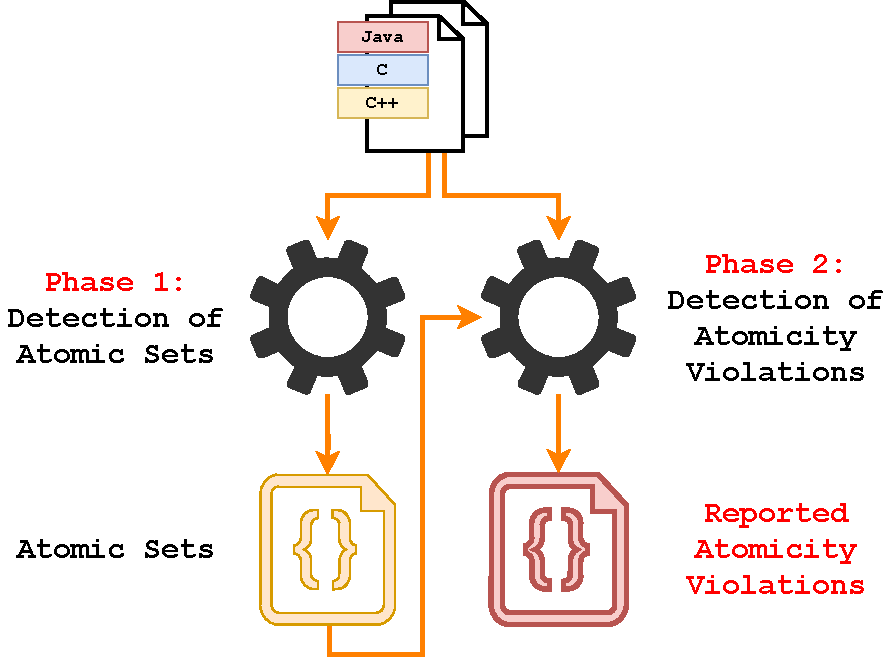
\includegraphics[width=.7 \linewidth]{analyser-proposal-sets.pdf}
\end{frame}


%%%%%%%%%%%%%%%%%%%%%%%%%%%%%%%%%%%%%%%%%%%%%%%%%%%%%%%%%%%%%%%%%%%%%%%%%%%%%%%%


\section{Phases of the Analysis (Approximated with Sets)}
\begin{frame}[fragile]{Phases of the Analysis (Approximated with Sets)}
    \setbeamercovered{transparent}
    \begin{columns}
        \begin{column}<1>[T]{.55 \linewidth}
            \begin{enumerate}
                \item Detection of \alert{atomic call sets}.
            \end{enumerate}

            \begin{itemize}
                \item \emph{Approximates} \alert{sequences by sets}.

                \item \textbf{Summary}: $ \chi \in \textcolor{magenta}{2^{2^\Sigma}} $
                    (\textcolor{magenta}{set of atomic call sets})
            \end{itemize}
            
            \hfill

\begin{lstlisting}
void f() {
  <@\texttt{\textcolor{red}{\textbf{lock}}}@>(L);
  x(); y(); z(); // x.y.z -> {x,y,z}
  <@\texttt{\textcolor{red}{\textbf{unlock}}}@>(L);
  a();
  <@\texttt{\textcolor{red}{\textbf{lock}}}@>(L);
  z(); y(); x(); // z.y.x -> {x,y,z}
  <@\texttt{\textcolor{red}{\textbf{unlock}}}@>(L);
}
\end{lstlisting}

            \hfill

            \centering
            \footnotesize

            $ \boldsymbol{\chi_\mathtt{f} = \textcolor{magenta}{\{\{\mathtt{x, y, z}\}\}}} $
            
            \hfill
        \end{column}

        \begin{column}<2>[T]{.45 \linewidth}
            \begin{enumerate}\setcounter{enumi}{1}
                \item Detection of \alert{atomicity violations}.
            \end{enumerate}

            \begin{itemize}
                \item Derives "\alert{atomic pairs}" from the first phase: $ \Omega \in 2^{\Sigma \times \Sigma} $.

                \item Looks for \emph{non-atomic pairs} of calls assumed to \alert{run atomically}.

                \item \textbf{Summary}: $ \chi \in \textcolor{orange}{2^{\Sigma \times \Sigma}} $ \\
                    (\textcolor{orange}{set of atomicity violations})
            \end{itemize}

            \hfill

\begin{lstlisting}
void g() {
  a(); <@\texttt{\textcolor{orange}{\textbf{x}}}@>(); <@\texttt{\textcolor{orange}{\textbf{y}}}@>(); b();
}
\end{lstlisting}

            \hfill

            \centering
            \footnotesize

            $ \boldsymbol{\Omega = \{(\mathtt{x, y}), (\mathtt{x, z}), (\mathtt{y, x}), (\mathtt{y, z}), (\mathtt{z, x}), (\mathtt{z, y})\}} $

            \smallskip

            $ (\mathtt{\textcolor{orange}{\boldsymbol{\mathtt{x}}}, \textcolor{orange}{\boldsymbol{\mathtt{y}}}}) \in \Omega \Longrightarrow \boldsymbol{\chi_\mathtt{g} = \textcolor{orange}{\{(\mathtt{x, y})\}}} $
        \end{column}
    \end{columns}
\end{frame}


%%%%%%%%%%%%%%%%%%%%%%%%%%%%%%%%%%%%%%%%%%%%%%%%%%%%%%%%%%%%%%%%%%%%%%%%%%%%%%%%


\section{Experimental Evaluation}
\begin{frame}{Experimental Evaluation}
    \begin{columns}
        \begin{column}{.45 \linewidth}
            \begin{itemize}\setlength\itemsep{1em}
                \item \alert{Scalability} evaluated on~54 \emph{real-life complex} C~programs.
                    \medskip
                    \begin{itemize}
                        \item 806,431 LOC in total.
                    \end{itemize}

                \item On average, \alert{twice faster}.
            \end{itemize}
        \end{column}

        \begin{column}{.55 \linewidth}
            \centering
            \begin{tabular}{|l|r|r|r|r|}
                \hline

                \multirow{2}{*}{} & \multicolumn{2}{c|}{\textbf{v1.0.0}} & \multicolumn{2}{c|}{\textbf{v2.0.0}} \\ \cline{2-5}

                & \textbf{Phs.~1} & \textbf{Phs.~2} & \textbf{Phs.~1} & \textbf{Phs.~2} \\ \hline \hline

                \textbf{Avg. Time (s)} & 70.98 & 109.11 & 37.96 & 50.93 \\ \hline

                \textbf{Total Time (s)} & 4,117 & 5,892 & 2,164 & 2,750 \\ \hline
            \end{tabular}
        \end{column}

        \hfill
    \end{columns}

    \vfill

    \begin{columns}
        \begin{column}{1.07 \linewidth}
            \begin{itemize}
                \item Experiments with \emph{Apache Cassandra} and \emph{Apache Tomcat} (both $ \sim $250 KLOC).
                    \bigskip
                    \begin{itemize}\setlength\itemsep{1.5em}
                        \item Successfully \alert{rediscovered} \emph{already fixed reported real bugs}.

                        \item The number of \emph{reported bugs} was \alert{significantly reduced} ($ \sim\!4\times $).

                        \item Still hard to say \emph{which of the bugs are real}\,---\,the \alert{accuracy} needs to be further improved.
                    \end{itemize}
            \end{itemize}
        \end{column}
    \end{columns}
\end{frame}


%%%%%%%%%%%%%%%%%%%%%%%%%%%%%%%%%%%%%%%%%%%%%%%%%%%%%%%%%%%%%%%%%%%%%%%%%%%%%%%%


\section{Summary}
\begin{frame}{Summary\footnotemark}
    \begin{itemize}\setlength\itemsep{.5em}
        \item \emph{Proposed} and \emph{implemented} \alert{extensions for Atomer}:
            \smallskip
            \begin{itemize}
                \item approximation with sets, support for C++ and Java, distinguishing different lock instances, parametrisation of the analysis.
            \end{itemize}

        \item Successfully \emph{tested} and \emph{experimentally evaluated}.
            \smallskip
            \begin{itemize}
                \item Both \emph{scalability} and \emph{accuracy} were \alert{significantly increased}.
            \end{itemize}

        \item Experiments with \emph{real-life programs}.
    \end{itemize}

    \medskip

    \textbf{Future goals}
    \smallskip
    \begin{itemize}
        \item Further increase \alert{accuracy}/reduce the number of \alert{false alarms}.
            \smallskip
            \begin{itemize}\setlength\itemsep{.5em}
                \item Combining with \emph{dynamic analysis}.

                \item \emph{Statistic ranking} of atomic functions/reported errors.

                \item Considering \emph{formal parameters} of functions.

                \item \emph{Machine learning} of analysis' parameter values.
            \end{itemize}
    \end{itemize}
    
    \footnotetext[1]{The preliminary results of this work were presented at the \emph{Excel@FIT’21} (\alert{won two awards}). It is supported by the \emph{H2020 ECSEL project VALU3S}.}
\end{frame}


%%%%%%%%%%%%%%%%%%%%%%%%%%%%%%%%%%%%%%%%%%%%%%%%%%%%%%%%%%%%%%%%%%%%%%%%%%%%%%%%


\appendix


%%%%%%%%%%%%%%%%%%%%%%%%%%%%%%%%%%%%%%%%%%%%%%%%%%%%%%%%%%%%%%%%%%%%%%%%%%%%%%%%


\section{Otázky oponenta}
\begin{frame}{Otázky oponenta}
    \begin{enumerate}
        \item \textbf{Plánujete podniknout další kroky pro zařazení \emph{Atomeru} do \alert{hlavní větve} frameworku \emph{Facebook Infer}?}
            \bigskip
            \begin{itemize}\setlength\itemsep{1.5em}
                \item \alert{Ano}, určitě bychom se rádi o~zařazení v~budoucnu pokusili. 

                \item Repositář Atomeru je \emph{pravidelně aktualizován na nejnovější verzi} frameworku.

                \item Atomer už byl dříve (úspěšně) \alert{presentován} a~\alert{konsultován} s~\emph{vývojáři Inferu}.
                    \medskip
                    \begin{itemize}
                        \item Presentace na \alert{Infer Practitioners Workshop} v~rámci konference \emph{PLDI 2020}.
                    \end{itemize}
            \end{itemize}
    \end{enumerate}
\end{frame}


%%%%%%%%%%%%%%%%%%%%%%%%%%%%%%%%%%%%%%%%%%%%%%%%%%%%%%%%%%%%%%%%%%%%%%%%%%%%%%%%


\section{Advanced Manipulation with Locks}
\begin{frame}{Advanced Manipulation with Locks}
    \begin{itemize}\setlength\itemsep{1.5em}
        \item \emph{Access path} used for a~\alert{lock's identification}: $ \pi \in \Pi \Coloneqq Var \times Field^* $,
            \smallskip
            \begin{itemize}\setlength\itemsep{.8em}
                \item $ Var $ is a~set of all variables,

                \item $ Field $ is a~set of field names.
            \end{itemize}

        \item Identification of a~\alert{critical section}: $ (\pi, l) \in \Pi \times \mathbb{N}^\top $,
            \smallskip
            \begin{itemize}\setlength\itemsep{.8em}
                \item $ \pi $ is an access path that identifies a~\emph{lock object} that locks the section,

                \item $ l $ is the \emph{number of locks} of the lock object identified by~$ \pi $,

                \item $ \mathbb{N}^\top $ denotes $ \mathbb{N} \cup \{\top\} $,
                    \smallskip
                    \begin{itemize}
                        \item $ \top $ represents a~number larger than some \alert{upper bound}~$ t \in \mathbb{N} $.
                    \end{itemize}
            \end{itemize}

        \item Representation of a~\alert{lock guard}: $ (\pi_g, L) \in \Pi \times 2^\Pi $,
            \smallskip
            \begin{itemize}\setlength\itemsep{.8em}
                \item $ \pi_g $ is an access path that identifies the lock guard,

                \item $ L $ is a~set of access paths that identify \emph{lock objects} associated with the guard.
            \end{itemize}
    \end{itemize}
\end{frame}


%%%%%%%%%%%%%%%%%%%%%%%%%%%%%%%%%%%%%%%%%%%%%%%%%%%%%%%%%%%%%%%%%%%%%%%%%%%%%%%%


\section{Facebook Infer's Architecture}
\begin{frame}{Facebook Infer's Architecture}
    \centering
    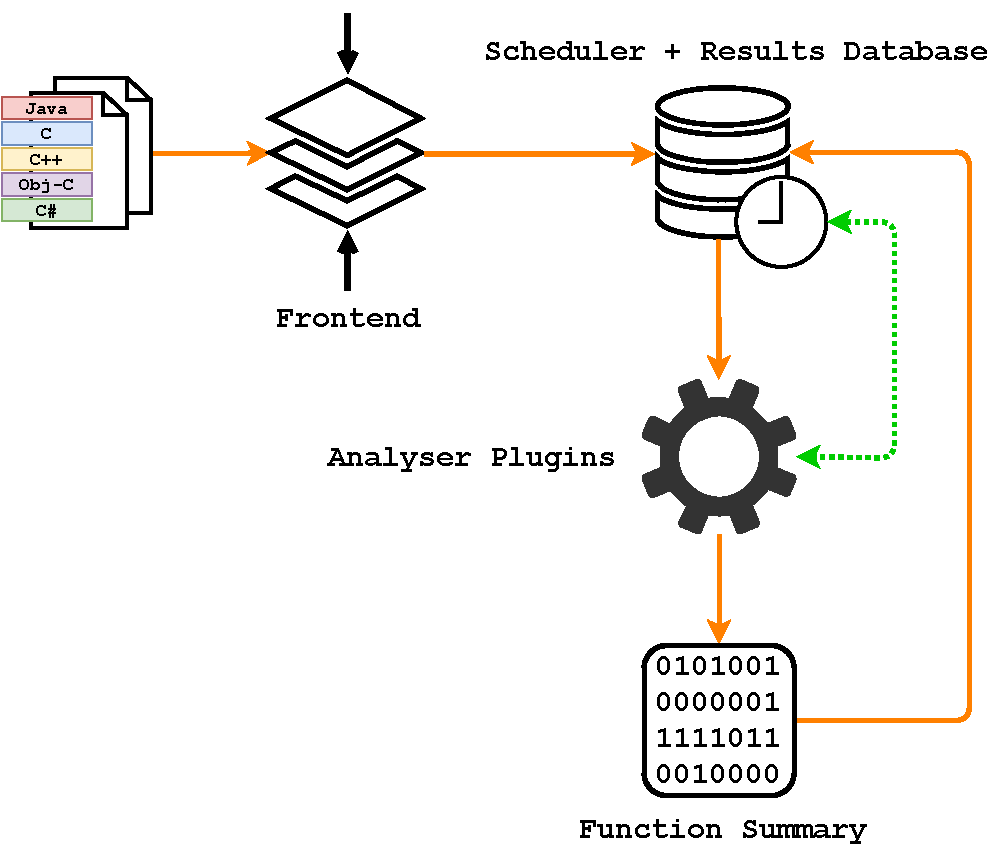
\includegraphics[width=.65 \linewidth]{infer-architecture.pdf}
\end{frame}


%%%%%%%%%%%%%%%%%%%%%%%%%%%%%%%%%%%%%%%%%%%%%%%%%%%%%%%%%%%%%%%%%%%%%%%%%%%%%%%%%


\section{Demonstration of Facebook Infer's Analysis}
\begin{frame}{Demonstration of Facebook Infer's Analysis}
    \centering
    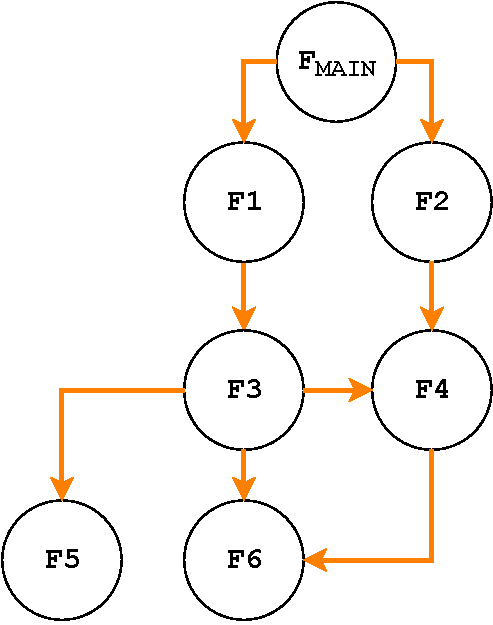
\includegraphics[width=.4 \linewidth]{infer-call-graph.pdf}
\end{frame}



%%%%%%%%%%%%%%%%%%%%%%%%%%%%%%%%%%%%%%%%%%%%%%%%%%%%%%%%%%%%%%%%%%%%%%%%%%%%%%%%%


\section{Abstract Interpretation in Facebook Infer}
\begin{frame}{Abstract Interpretation in Facebook Infer}
    \centering
    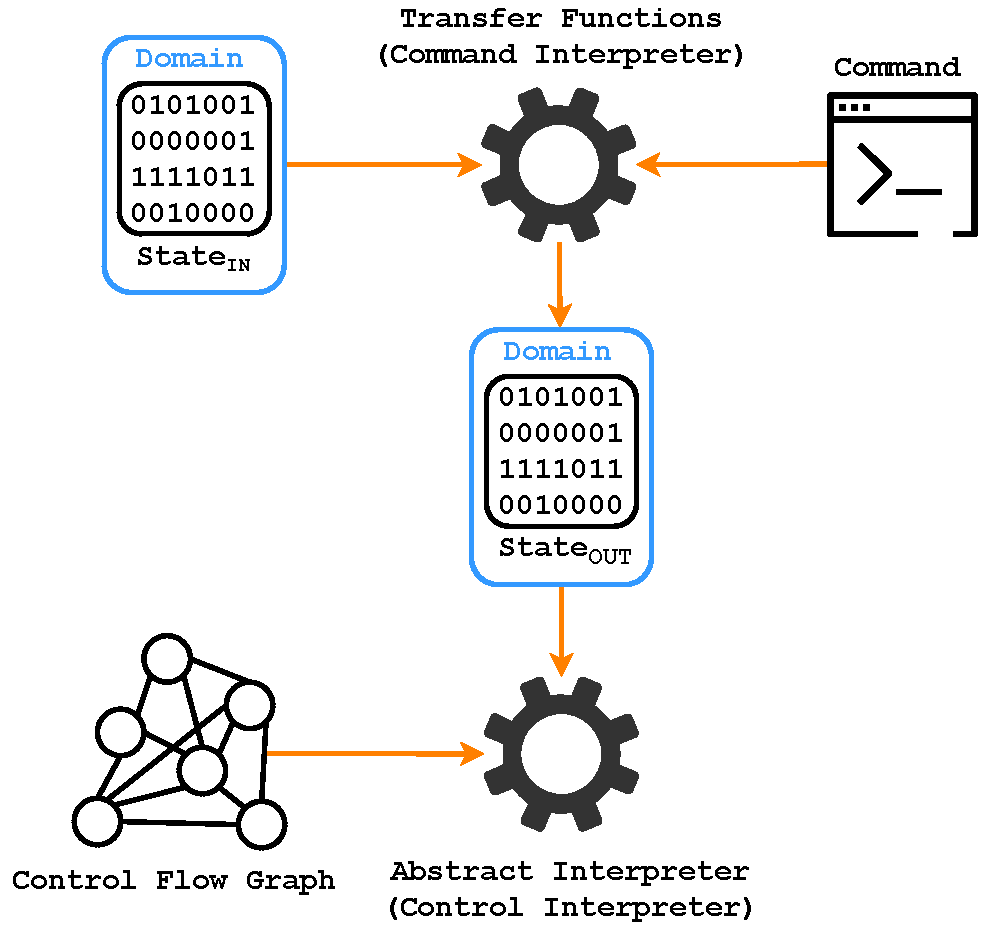
\includegraphics[width=.58 \linewidth]{infer-analysis.pdf}
\end{frame}


%%%%%%%%%%%%%%%%%%%%%%%%%%%%%%%%%%%%%%%%%%%%%%%%%%%%%%%%%%%%%%%%%%%%%%%%%%%%%%%%


\section{Rediscovered Bug in Apache Tomcat}
\begin{frame}[fragile]{Rediscovered Bug in Apache Tomcat}
    \alert{Real-life bug} in a~package \texttt{\textbf{org.apache.catalina.core.StandardContext}}

    \medskip

\begin{lstlisting}[language=java, morekeywords={String}]
public void addParameter(String name, String value) {
  <@\texttt{\ldots}@>
  if (parameters.get(name) != null)
    throw new IllegalArgumentException
      (sm.getString("standardContext.parameter.duplicate", name));

  // Add this parameter to our defined set
  synchronized (parameters) {
    parameters.put(name, value);
  }
  fireContainerEvent("addParameter", name);
}
\end{lstlisting}
\end{frame}


%%%%%%%%%%%%%%%%%%%%%%%%%%%%%%%%%%%%%%%%%%%%%%%%%%%%%%%%%%%%%%%%%%%%%%%%%%%%%%%%


\end{document}
